\documentclass{beamer}

 \usepackage[german]{babel}
 \usepackage[utf8]{inputenc}
 \usepackage{graphicx}
\usetheme{Antibes}

\setbeamercovered{transparent}
\beamertemplatenavigationsymbolsempty
\setbeamertemplate{footline}[frame number]
\title[Raspberry Pi ROS \hspace{3cm} Denis Herdt, Almin Causevic]{Raspberry Pi ROS}
\author{Denis Herdt, Almin Causevic}
\institute[I_HS Wgt-Rav]{Angewandte Informatik HS Weingarten-Ravensburg}
\date{\today}
%\logo{\pgfimage[width=2cm,height=2cm]{hulogo}}
%\titlegraphic{\includegraphics[width=2cm,height=2cm]{hulogo}}
\subject{Raspberry Pi ROS}

\begin{document}
\frame{\titlepage}

\begin{frame}
{\bf Ablauf}
\begin{enumerate}
\item Motivation
\item ROS Grundlagen
\item Implementation Netzwerk
\item Anwendung Volksbot
\item Fazit
\end{enumerate}
\end{frame}

\begin{frame}
{\bf Motivation}
\centerline{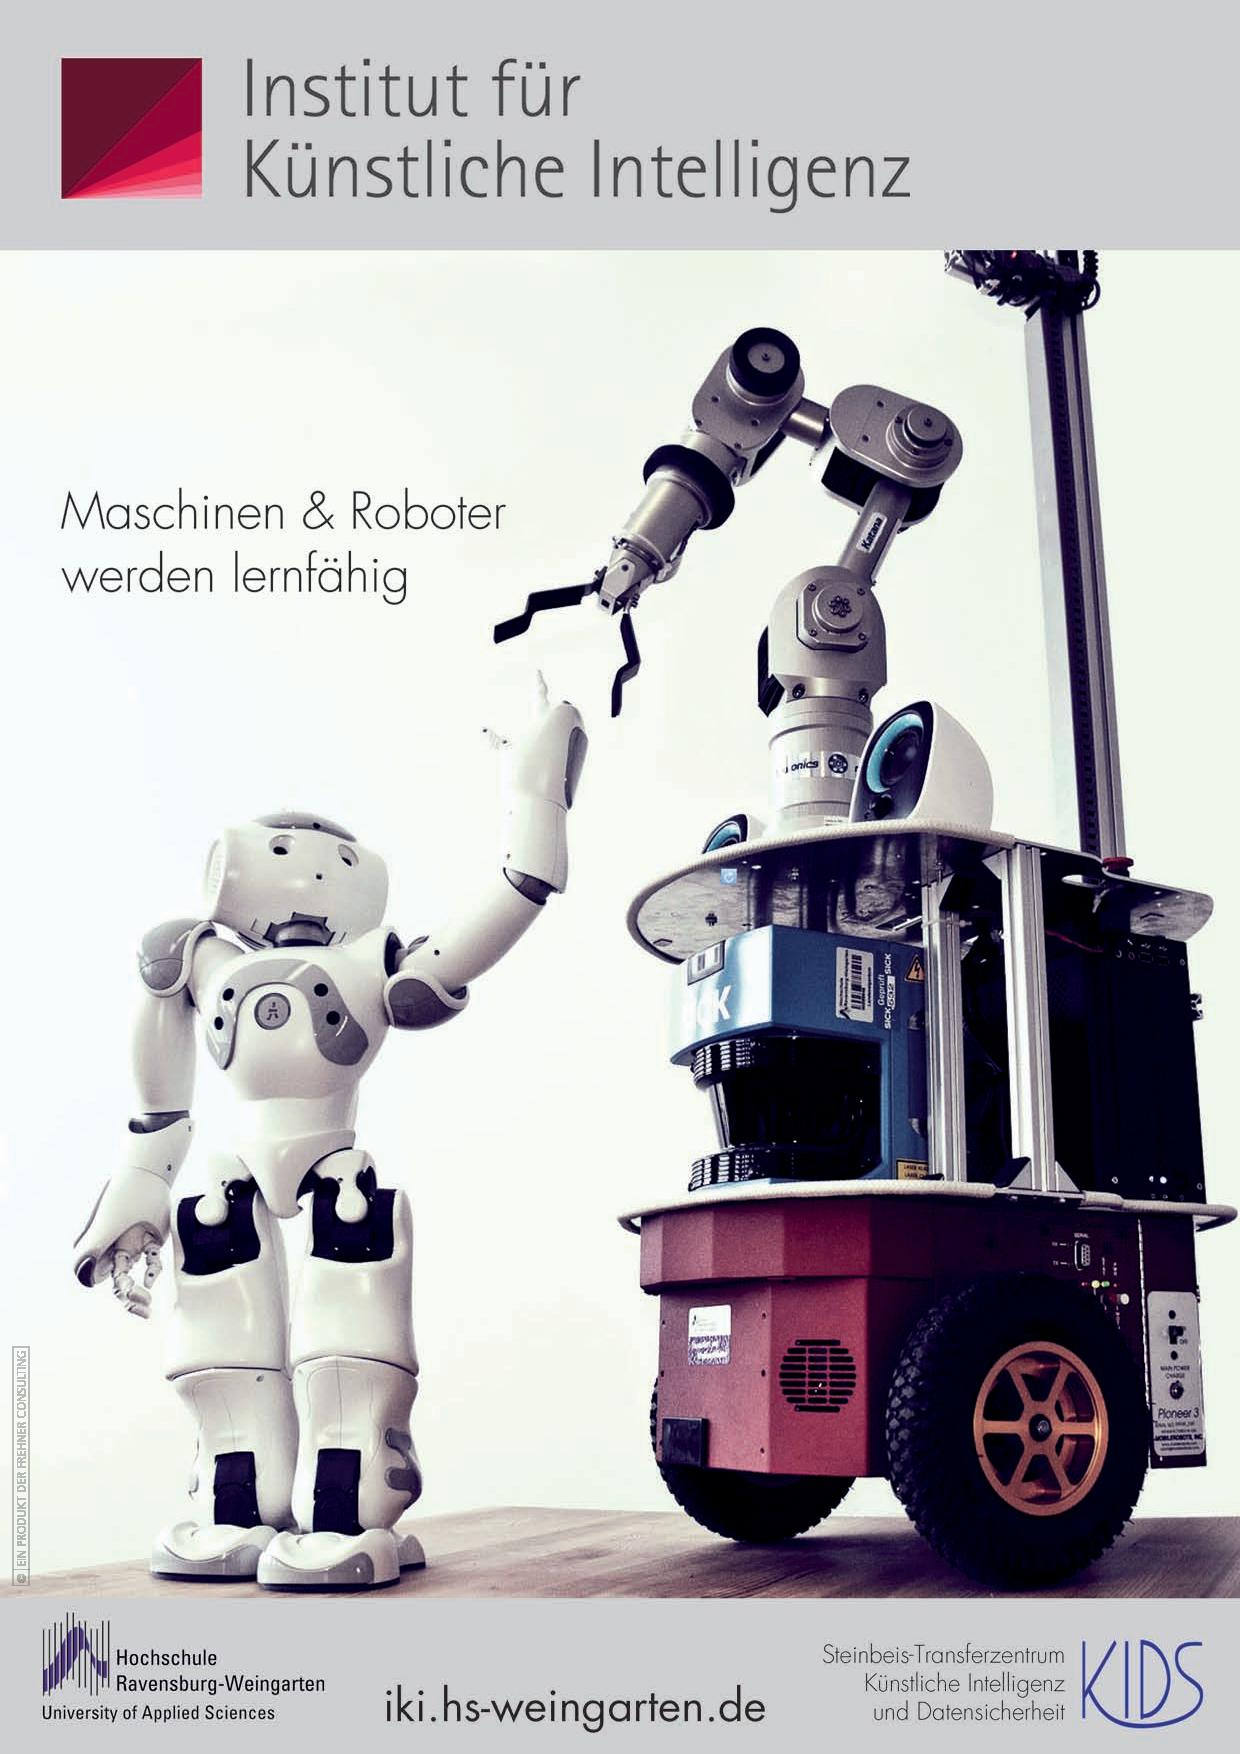
\includegraphics[width=6cm]{pics/iki.jpg}}\cite{iki}
\end{frame}

\begin{frame}
{\bf ROS Grundlagen}
\centerline{
\includegraphics[width=9cm]{pics/ros5.png}}\cite{ros5}
\end{frame}

\begin{frame}
\centerline{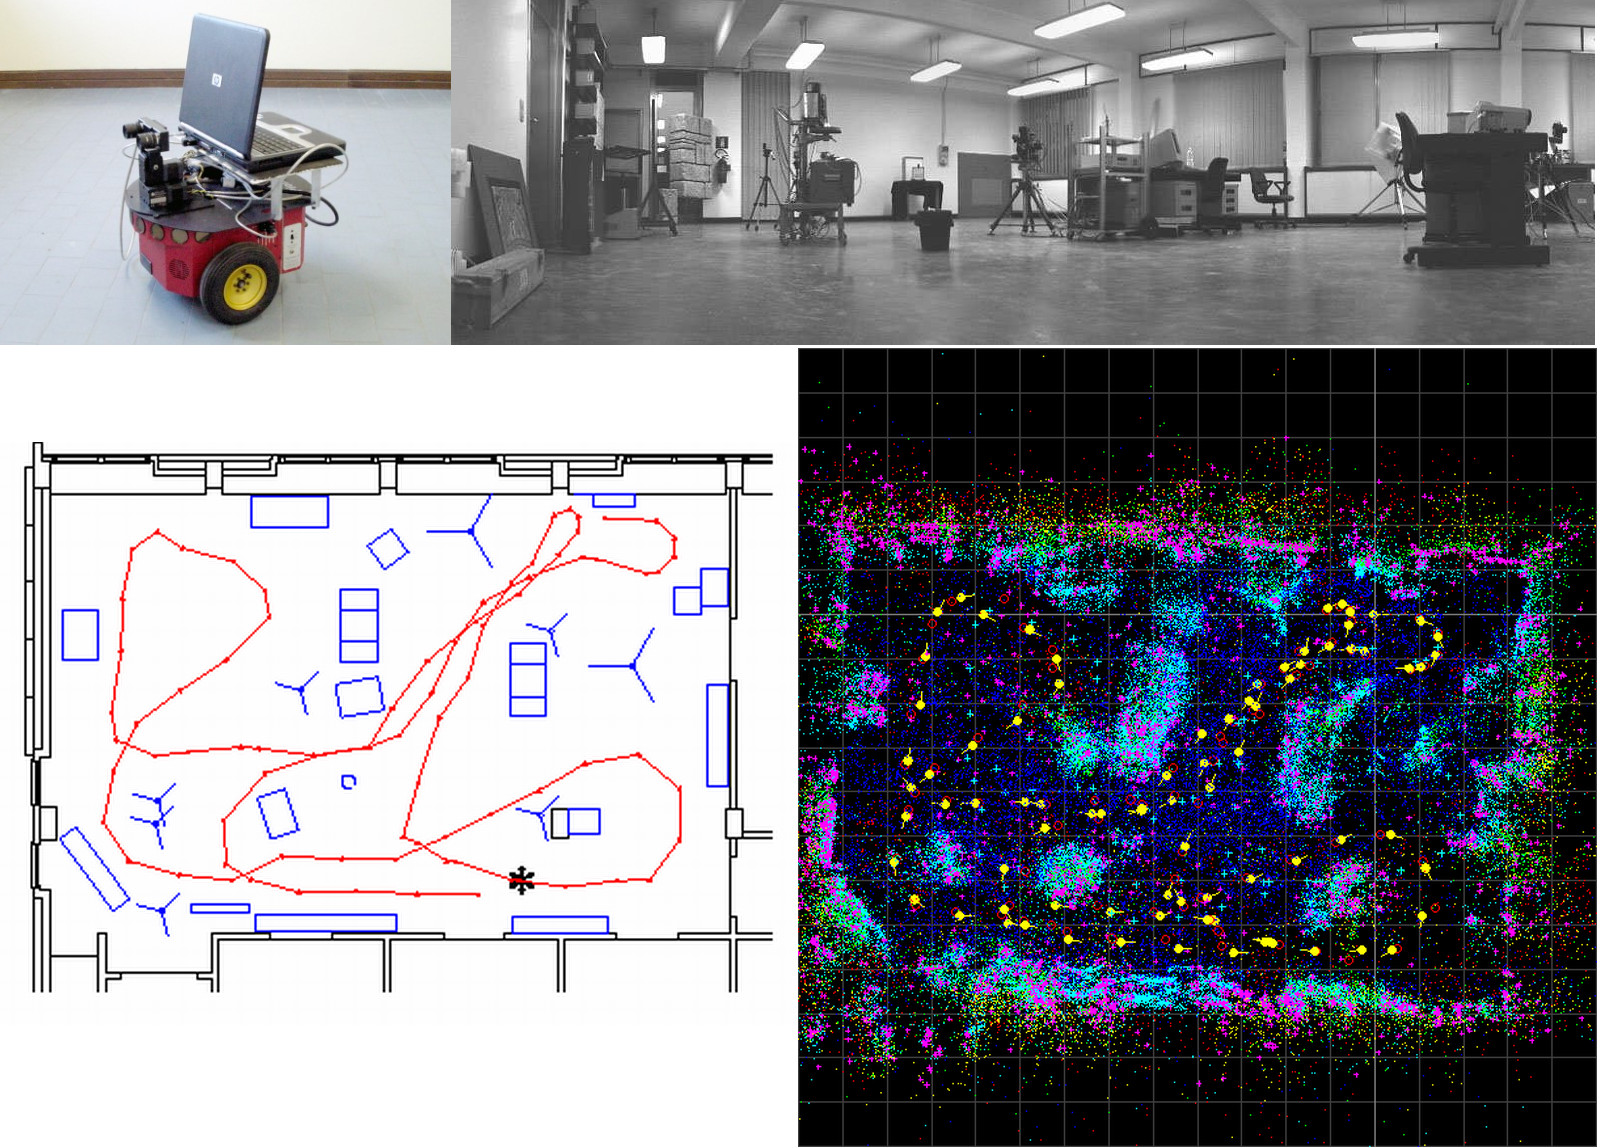
\includegraphics[width=9cm]{pics/slam.png}}\cite{slam}
\end{frame}

\begin{frame}
\centerline{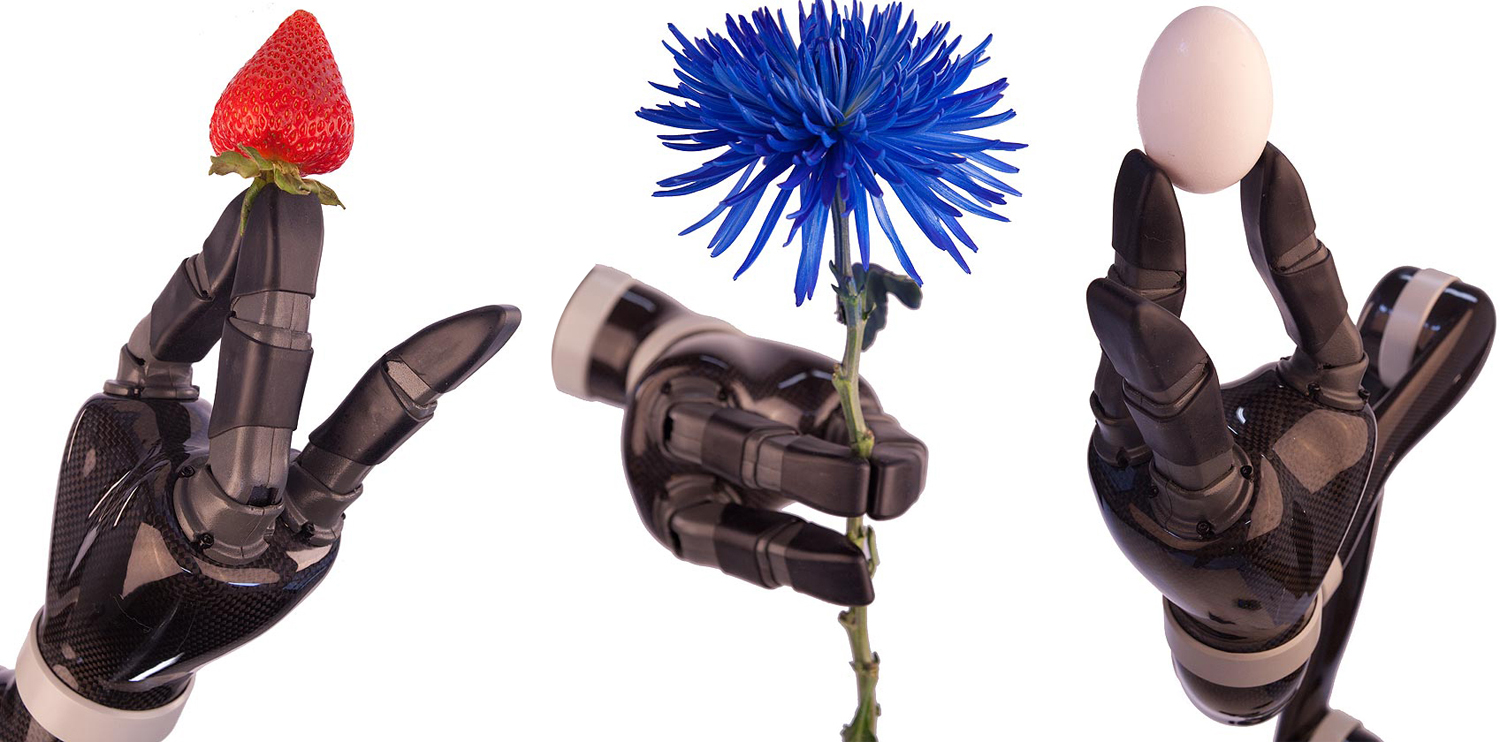
\includegraphics[width=9cm]{pics/jaco_arm.jpg}}\cite{arm}
\end{frame}

\begin{frame}
\huge Alternativen? \\
\parbox{4cm}{
\includegraphics[width=3cm]{pics/carmen.png}}\cite{carmen}
\parbox{4cm}{
\includegraphics[width=3cm]{pics/yarp.png}}\cite{yarp}
\parbox{4cm}{
\includegraphics[width=3cm]{pics/microsoft.jpg}}\cite{microsoft}
\hspace{4cm}
\parbox{4cm}{
\includegraphics[width=3cm]{pics/orocos.jpg}}\cite{orocos}
\parbox{4cm}{
\includegraphics[width=3cm]{pics/orca.png}}\cite{orca}
\end{frame}

\begin{frame}
\centerline{
\includegraphics[width=4cm]{pics/ros_equation1.png}}
\centerline{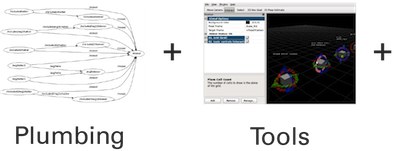
\includegraphics[width=6cm]{pics/ros_equation2.png}}
\centerline{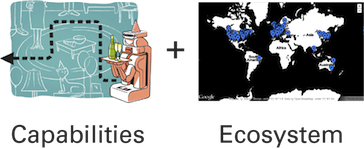
\includegraphics[width=6cm]{pics/ros_equation3.png}}\cite{equation}
\end{frame}

\begin{frame}
\centerline{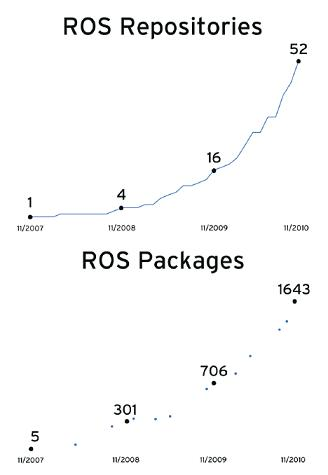
\includegraphics[width=6cm]{pics/ros_repos.jpg}}\cite{repos}
\end{frame}


\begin{frame}
{\bf Implementation Netzwerk}
\parbox{4cm}{
\includegraphics[width=6cm]{pics/pilogo.png}}
\hspace{0.5cm} 
$\rightarrow$
\parbox{4cm}{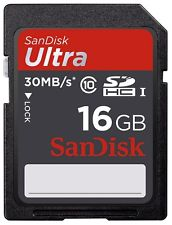
\includegraphics[width=3cm]{pics/sd.jpg}}\cite{sd}
\end{frame}


\begin{frame}
\centerline{
\includegraphics[width=5.5cm]{pics/groovy.jpg}}\cite{groovy}
\end{frame}

\begin{frame}
{\bf Fazit}
\centerline{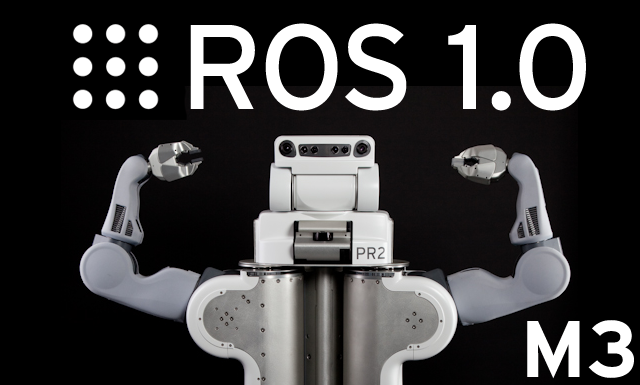
\includegraphics[width=6cm]{pics/ros.png}}\cite{ros}
\end{frame}

\begin{frame}
\centerline{
\includegraphics[width=4cm]{pics/goku.jpg}}\cite{goku}
\vspace{2cm}
\centerline{{\bf \Huge FRAGEN?}}
\end{frame}

\end{document}
%groovy http://www.ros.org/news/announcements/
%sd http://www.gadgetsok.com/free-shipping-sandisk-16gb-sd-card-class-10-30m-$
%repos http://www.ros.org/news/2010/11/
%equation http://www.ros.org/about-ros/
%orca http://orca-robotics.sourceforge.net/
%orocos http://www.orocos.org/
%yarp http://wiki.icub.org/yarp/
%carmen http://www.ual.es/personal/rgonzalez/english/materials.htm
%microsoft http://mydreamsinside.blogspot.de/2010_12_01_archive.html
%arm http://www.robotshop.com/blog/en/jaco-the-new-robotic-manipulator-arm-by$
%slam http://einsteinbots.blogspot.de/2011/07/slam.html
%ros5 http://www.instructables.com/id/Getting-Started-with-ROS-Robotic-Operat$
%fragen http://www.hs-weingarten.de/web/iaf-institut-fuer-angewandte-forschun$
%iki http://iki.hs-weingarten.de/?lang=de&page=s_broschuere
%ros http://www.willowgarage.com/blog/2010/01/22/milestone-3-complete-pr2-betas-ready-and-ros-10